\scanpage{20}
% L1–2
2) Déterminer les classes à \unsure{isomorphismes|isomorphisme} près d'espaces \deleted{fibrés} principaux homogènes sous $B$.

% L3, divider
\figure{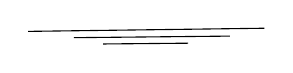
\begin{tikzpicture}\draw (0,0)--(3,.04) (.58,-.08)--(2.56,-.06) (.95,-.16)--(2.03,-.15);\end{tikzpicture}}

% L4–6
Soit $C$ une $A$-algèbre \inserted{libre de rang $p$}, munie d'une $A$-dérivation $D$ telle que $D^p=0$, et que les $D^i$ $(0\leq i\leq p-1)$ forment une \uline{base} de $\operatorname{Hom}_A(C,C)$ sur $C$.
% L7–8
Alors l'\uline{ensemble des éléments} \uline{de} $C$ \uline{annulés par} $D$ \uline{est $A$}. \deleted{\illegible{1}}
% slanted
\margin{autre \unsure{démonstration} : on étend les \unsure{scalaires} de $A$ à $C$.}
En effet, tout sous-$A$-module $M$ de $C$ qui est \inserted{libre de rang $m$ et} facteur direct \deleted{$\unsure{x}$} dans $C$,
% L10–12
est identique à l'ensemble $(M^\circ)^\circ$ des zéros de l'ens. $M^\circ$ des $v\in\operatorname{Hom}(C,C)$ qui s'annulent sur $M$ (\unsure{immédiat|évident}), et $M^\circ$ est un sous $C$-module libre de rang $p-m$ dans $\deleted{\unsure{C^p}}\operatorname{Hom}(C,C)$,
% L13–15
\deleted{\unsure{qui}} qui est facteur direct de ce sous-$C$-module\,; par suite\,; \uline{si}
% slanted
\margin{\uline{Lemme} à développer}
% L16–18
on a $p-m$ éléments $u_i$ dans $M^\circ$ qui \deleted{\unsure{engendrent un}} \inserted{forment la base d'un} sous-module \deleted{libre de rang \unsure{$p-m$} de \unsure{$K|C$}} \inserted{$L$ de $\operatorname{Hom}(C,C)$} qui est facteur direct,
% L19–21
alors nécessairement $L=M^\circ$, d'où $M=L^\circ$, i.e. $M$ est l'ens des éléments de $C$ annulés par les $u_i$. On applique ceci
% archive sheet number: 19
